\graphicspath{{images/university/}}
\section{Об университете}
	Раздел позволяет просматривать и редактировать информацию, связанную с университетом: основную информацию, контакты, а также медиа"=файлы, отвечающие за отображение страниц, связанных с этим вузом на сайте.
	
	\subsection{Роли и операции}
	
	Раздел доступен пользователям, имеющим следующие роли:	

	\begin{itemize}
		\item Администратор Платформы:
		\begin{itemize}
			\item просмотр информации об университете;
			\item редактирование информации об университете;
			\item создание нового университета.
		\end{itemize}
		\item Администратор вуза"=поставщика:
		\begin{itemize}
			\item просмотр информации об университете;
			\item редактирование информации об университете.
		\end{itemize}
		\item Администратор контента вуза"=поставщика:
		\begin{itemize}
			\item просмотр информации об университете;
			\item редактирование информации об университете.
		\end{itemize}
	\end{itemize} 
	
	\subsection{Просмотр информации об университете}\label{university:detail_section}
	При выборе в главном меню пункта \quotes{Об университете} загружается подраздел \quotes{Просмотр информации}, в котором доступны для просмотра все имеющиеся на текущий момент данные об университете.

	Внешний вид подраздела приведён на рисунке~\ref{university:detailview}
	
	\begin{figure}[H]
	\center{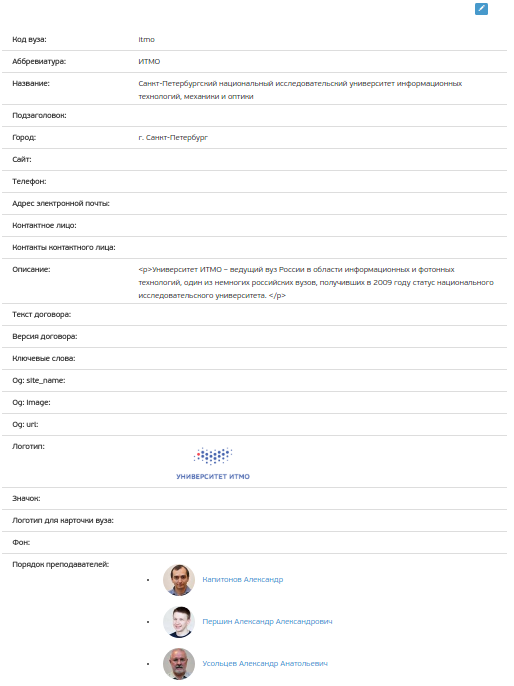
\includegraphics[width=1\linewidth]{detailview.png}}
	\caption{Внешний вид подраздела \quotes{Просмотр информации}}
	\label{university:detailview}
	\end{figure}
	
	Для просмотра доступны следующие поля:
	\begin{itemize}
		\item код вуза "--- уникальный код университета на Платформе, заполняется при создании вуза, неизменяем;
		\item аббревиатура;
		\item полное название университета;
		\item подзаголовок "--- краткое название университета;
		\item город;
		\item сайт;
		\item телефон;
		\item e"=mail;
		\item контактное лицо по умолчанию для связи по договорам, заключаемым данным университетом;
		\item контакты контактного лица (e"=mail, номер телефона, др.);
		\item описание университета;
		\item текст договора, согласие с которым должен подтвердить студент для того, чтобы получить доступ к курсам данного университета;
		\item версия договора, с которым соглашается студент при записи на курс;
		\item метаданные: ключевые слова, og:site\_name, og:image, og:url;
		\item логотип университета;
		\item значок;
		\item логотип для карточки вуза;
		\item фон;
		\item порядок преподавателей "--- список преподавателей в том порядке, в котором они будут показываться на странице университета на сайте, элемент списка "--- ссылка, ведущая на страницу просмотра подробной информации о конкретном преподавателе.
	\end{itemize}

	\subsection{Редактирование информации об университете}\label{university:edit}
	Для перехода к подразделу редактирования необходимо нажать на иконку \quotes{редактирование} \vcenteredinclude[width=0.1\linewidth]{edit_icon.png} в верхнем правом углу страницы подраздела \quotes{Просмотр информации} (рис.~\ref{university:detailview}).

	
	В этом случае осуществляется переход к форме редактирования университета, в которой можно изменять поля, описанные в разделе~\ref{university:detail_section}. 
	
	\subsubsection{Поля и ошибки}
	В форме представлено несколько типов полей:
	\begin{itemize}
		\item \textbf{Обязательные поля} отмечены символом \quotes{*}, если такое поле оставить не заполненным "--- появляется сообщение о необходимости его заполнения и блокируется кнопка сохранения изменений (см. рис.~\ref{university:edit_required}).
		
		\begin{figure}[H]
		\center{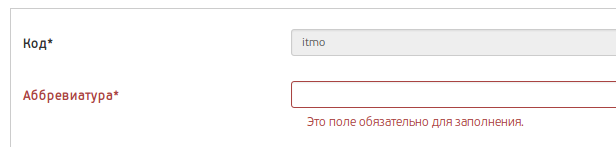
\includegraphics[width=1\linewidth]{edit_required.png}}
		\caption{Обработка заполнения обязательных полей}
		\label{university:edit_required}
		\end{figure}	
	
		\item \textbf{Сайт и адрес электронной почты университета}. Ввод информации в эти поля необходимо осуществлять в корректном формате, например, \texttt{http://npoed.ru} для сайта и \texttt{npoed@mail.ru} для почты соответственно, в противном случае появится сообщение об ошибке и будет заблокирована кнопка сохранения изменений (см. рис.~\ref{university:edit_url_email})
		
		\begin{figure}[H]
		\center{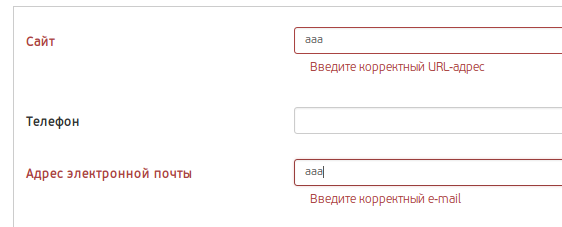
\includegraphics[width=1\linewidth]{edit_url_email.png}}
		\caption{Обработка заполнения полей \quotes{Сайт} и \quotes{Адрес электронной почты}}
		\label{university:edit_url_email}
		\end{figure}	
		
		\item \textbf{Поле \quotes{порядок преподавателей}} представляет собой список ФИО преподавателей университета в том порядке, в котором они будут показаны на сайте. Описание работы с виджетом изменения порядка см. в подразделе~\ref{widget:ordering}

		Для каждого преподавателя отдельно можно настроить его видимость на сайте в подразделе редактирование преподавателя путем переключения значения поля \quotes{Опубликован}, неопубликованные преподаватели скрыты на сайте для пользователей. В форме редактирования университета в списке преподавателей показываются как скрытые, так и опубликованные преподаватели. В зависимости от статуса их ФИО имеют различный цвет. Подробное описание можно получить, нажав на иконку \quotes{помощь} рядом с меткой поля (см. рис.~\ref{university:edit_instructors_legend}).
		
		\begin{figure}[H]
		\center{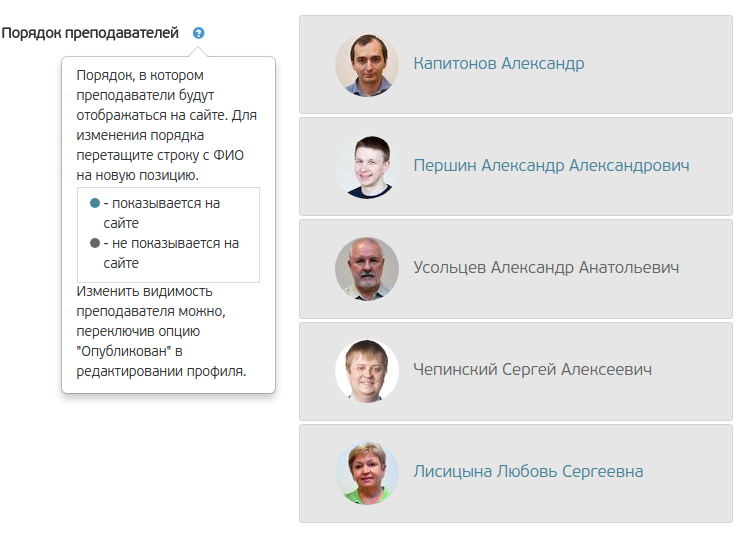
\includegraphics[width=1\linewidth]{edit_instructors_legend.png}}
		\caption{Справка о статусе преподавателей}
		\label{university:edit_instructors_legend}
		\end{figure}	
		
		\item \textbf{Файлы}. Форма редактирования позволяет загружать изображения для формирования внешнего вида страницы университета на сайте. Слева под меткой поля показано текущее загруженное изображение, если оно есть (см рис.~\ref{university:edit_logo}) или изображение по умолчанию, если ничего не загружено (см рис.~\ref{university:edit_icon_image}). Подробная информация по работе с файловыми полями приведена в разделе~\ref{widget:file_upload}.

		\begin{figure}[H]
		\center{
\includegraphics[width=1\linewidth]{edit_logo.png}}
		\caption{Файловое поле с загруженным изображением}
		\label{university:edit_logo}
		\end{figure}	
		
		\begin{figure}[H]
		\center{
\includegraphics[width=1\linewidth]{edit_icon_image.png}}
		\caption{Файловое поле с изображением по умолчанию}
		\label{university:edit_icon_image}
		\end{figure}
\end{itemize}

	\subsubsection{Элементы управления}\label{university:edit_save_cancel}
Управление внесенными изменениями осуществляется с помощью кнопок, расположенных внизу страницы (см. рис.~\ref{university:edit_buttons}).
		\begin{figure}[H]
		\center{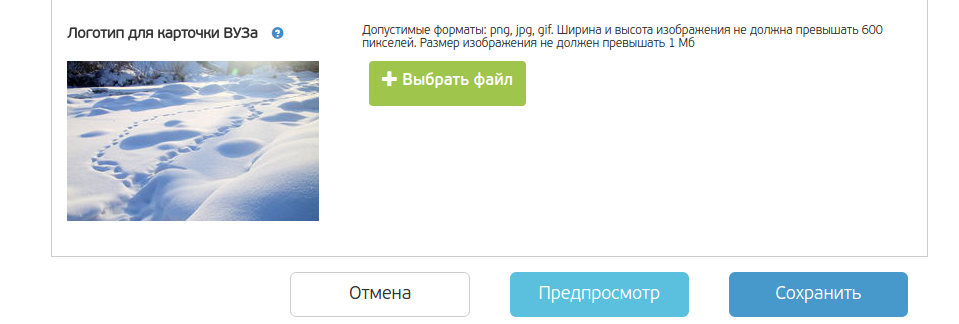
\includegraphics[width=1\linewidth]{edit_buttons.png}}
		\caption{Элементы управления подраздела редактирования}
		\label{university:edit_buttons}
		\end{figure}	
		
При нажатии \quotes{сохранить} осуществляется попытка сохранения формы: если форма заполнена корректно, то внесенные изменения сохраняются, пользователь перенаправляется в раздел \quotes{просмотр информации об университете}, в противном случае, если имеются ошибки, отображаются сообщения об ошибках, осуществляется прокрутка к месту первой ошибки. 


При нажатии кнопки \quotes{отмена} все изменения теряются, пользователь перенаправляется на предыдущую страницу.


Действия, вызываемые по нажатию кнопки \quotes{предпросмотр}, описаны в разделе~\ref{university:edit_preview_ch}
	
	\subsubsection{Предпросмотр}\label{university:edit_preview_ch}
	Для подраздела \quotes{Редактирование университета} доступна опция предпросмотра, с помощью которой можно оценить внешний вид страницы университета на сайте для пользователей с учётом внесенных изменений. Предпросмотр можно осуществить даже в том случае, если форма заполнена некорректно или не полностью. Страница загружается во всплывающем окне при нажатии кнопки \quotes{Предпросмотр} внизу страницы с формой редактирования (см. рис.~\ref{university:edit_preview}). При этом все внешние ссылки на отображаемой странице заблокированы.
	
		\begin{figure}[H]
		\center{
\includegraphics[width=1\linewidth]{edit_preview.png}}
		\caption{Окно предпросмотра}
		\label{university:edit_preview}
		\end{figure}	

Закрыть окно предпросмотра можно нажатием за пределы окна, либо по нажатию кнопки \quotes{закрыть} внизу окна, либо по нажатию крестика [х] в верхнем правом углу окна. Также из окна можно осуществить попытку сохранения внесенных изменений путем нажатия на кнопку \quotes{сохранить} в нижней части окна (см. рис.~\ref{university:edit_preview_button}). При этом поведение будет такое же, как при попытке сохранения из формы редактирования (см.~\ref{university:edit_save_cancel}).

		\begin{figure}[H]
		\center{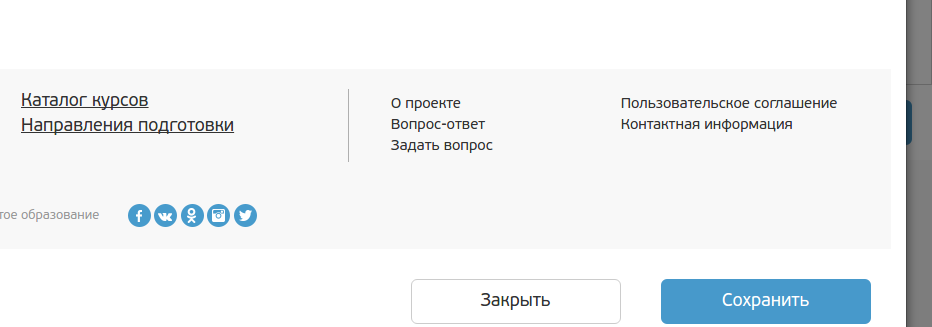
\includegraphics[width=1\linewidth]{edit_preview_button.png}}
		\caption{Элементы управления окна предпросмотра}
		\label{university:edit_preview_button}
		\end{figure}	
		
\subsection{Создание университета}
Возможность создания кабинета университета доступна администратору Платформы. 

Для перехода в подраздел необходимо выбрать в меню \quotes{Мой профиль}, расположенном в верхнем правом углу страницы, пункт \quotes{добавить вуз} (см. рис.~\ref{university:create_menu}).

		\begin{figure}[H]
		\center{
\includegraphics[width=1\linewidth]{create_menu.png}}
		\caption{Выбор пункта \quotes{Добавить вуз} в меню пользователя}
		\label{university:create_menu}
		\end{figure}	
		
В этом случае осуществляется переход к форме создания университета, в которой возможно задать значения полей, описанных в разделе~\ref{university:detail_section}. Содержание, возможные действия и реакции в этом разделе аналогичны описанным в разделе \quotes{Редактирование информации об университете}~\ref{university:edit} за исключением двух моментов:
\begin{itemize}
	\item В форме создания задается уникальный код университета на Платформе (поле \quotes{Код}), который в последствие не может быть изменен. При нажатии на поле ввода появляется подсказка о требуемом формате кода (см. рис.~\ref{university:create_slug_help}). При несоответствии введенного кода этому формату появится сообщение об ошибке. Также необходимым условием валидности кода является его уникальность, при наборе уже существующего на Платформе значения появится сообщение об ошибке (см. рис.~\ref{university:create_slug_exist}). Поле \quotes{Код} является обязательным.
	
		\begin{figure}[H]
		\center{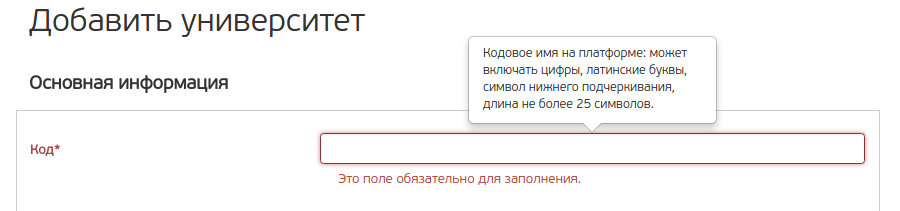
\includegraphics[width=1\linewidth]{create_slug_help.png}}
		\caption{Сообщение"=подсказка о формате кода университета}
		\label{university:create_slug_help}
		\end{figure}
		
		\begin{figure}[H]
		\center{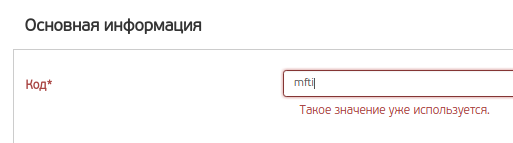
\includegraphics[width=1\linewidth]{create_slug_exist.png}}
		\caption{Сообщение об ошибке: введенный код уже занят}
		\label{university:create_slug_exist}
		\end{figure}	
		
	\item Вторым отличием от формы редактирования является отсутствие списка преподавателей. Они добавляются после создания университета через раздел \quotes{Преподаватели}, и после добавления отображаются в разделах \quotes{Просмотр информации об университете}, \quotes{Редактирование университета}, \quotes{Преподаватели}.
\end{itemize}
	
	

		

	
	
	
	
	
	